\begin{center}
{\textbf{Dimanche 22 août : Les nouveaux animatheurs entrent en action !}}
\end{center}
\vspace{2mm}

Benoît est le dernier animatheur de la seconde période à nous rejoindre et l’équipe est de nouveau au complet. De nouveau, une journée remplie attend les élèves. Baptiste et Colin enseignent la géométrie aux groupes C et D. De leur côté, Vladimir et Yaël donnent leur tout premier cours respectivement aux groupes A et B le matin !

\begin{figure}[H]
\centering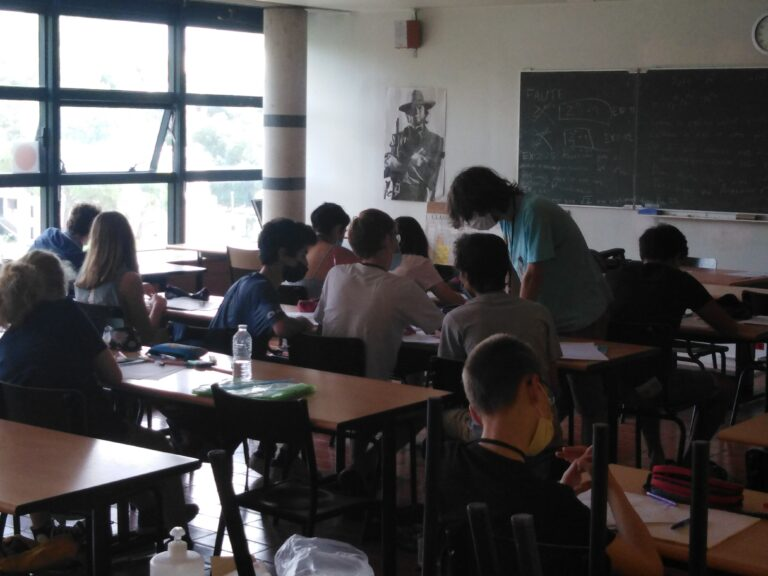
\includegraphics[height=7cm]{CR-22-0.jpg}\hspace{2cm}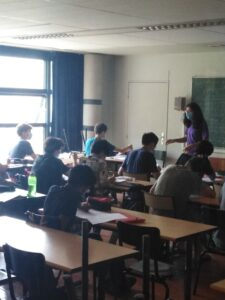
\includegraphics[height=7cm]{CR-22-1.jpg}
\caption{Quoi de mieux que les nombres premiers pour un premier cours avec Vladimir ! Attention, en groupe B, les profs sont pris en otage par les élèves pendant la pause de midi…}
\end{figure}

Après un repas (rapide pour ceux dont le cours a duré plus longtemps que prévu !), les cours de l’après-midi reprennent. C’est un après-midi combinatoire qui attend trois des quatre groupes avec respectivement Maena qui enseigne les invariants (et déborde un peu sur d’autres notions…) au groupe A, Savinien les pavages et coloriages (ce n’est pas aussi simple que ça en a l’air !) au groupe B et Emile la géométrie combinatoire au groupe D. En parallèle, Matthieu organise une formation pour les nouveaux animatheurs.

\begin{figure}[H]
\centering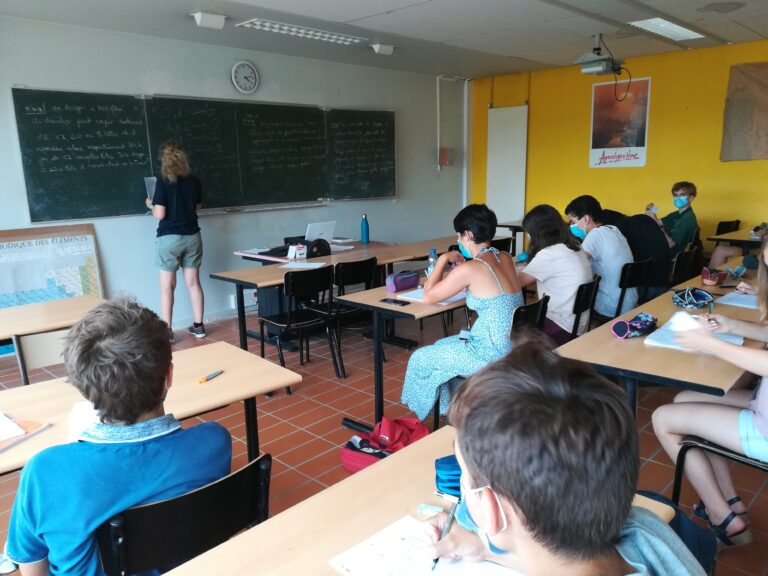
\includegraphics[width=6cm]{CR-22-2.jpg}
\caption{Maena délègue le travail en envoyant les élèves corriger les exercices au tableau.}
\end{figure}

A 16h30 + epsilon, les élèves sont enfin libérés et peuvent profiter soit des activités sportives (foot et volley) organisées par Colin et Baptiste, soit des nombreux jeux de société mis à disposition. C’est une soirée tranquille qui se profile pour les élèves (et plus studieuse pour les animatheurs qui planchent déjà sur la préparation du nouvel entraînement).

\begin{figure}[H]
\centering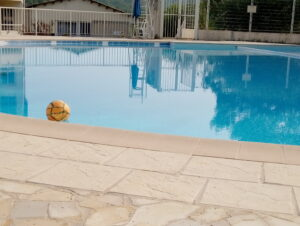
\includegraphics[width=6cm]{CR-22-3.jpg}\hspace{2cm}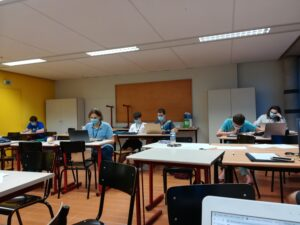
\includegraphics[width=6cm]{CR-22-4.jpg}
\caption{Un malheureux ballon a atterri dans la piscine après une partie de foot emballée. Ambiance sérieuse en salle des anims…}
\end{figure}